\documentclass[a4paper]{article}

\usepackage[czech]{babel} %https://github.com/michal-h21/biblatex-iso690
\usepackage[
   backend=biber      % if we want unicode 
  ,style=iso-numeric % or iso-numeric for numeric citation method          
  ,babel=other        % to support multiple languages in bibliography
  ,sortlocale=cs_CZ   % locale of main language, it is for sorting
  ,bibencoding=UTF8   % this is necessary only if bibliography file is in different encoding than main document
]{biblatex}

\usepackage[utf8]{inputenc}
\usepackage{fancyhdr}
\usepackage{amsmath}
\usepackage{amssymb}
\usepackage[left=2cm,right=2cm,top=2.5cm,bottom=2.5cm]{geometry}
\usepackage{graphicx}
\usepackage{pdfpages}
\usepackage{url}
\usepackage{import}
\usepackage{siunitx}
\sisetup{locale = DE}  %, separate-uncertainty = true    kdybych chtel +/-

\usepackage{float}
\newfloat{graph}{htbp}{grp}
\floatname{graph}{Graf}
\newfloat{tabulka}{htbp}{tbl}
\floatname{tabulka}{Tabulka}

\newcommand{\chyba}[3]{(\num{#1}\pm\num{#2}^{\text{stat}}\pm\num{#3}^{\text{sys}})\cdot\SI{e11}{\coulomb\per\kg}}
\renewcommand{\thefootnote}{\roman{footnote}}

\pagestyle{fancy}
\lhead{Praktikum IV - (A23) Určení měrného náboje elektronu z trajektorie ve zkřížených polích}
\rhead{Vladislav Wohlrath}
\author{Vladislav Wohlrath}

\bibliography{source}

\begin{document}

\begin{titlepage}
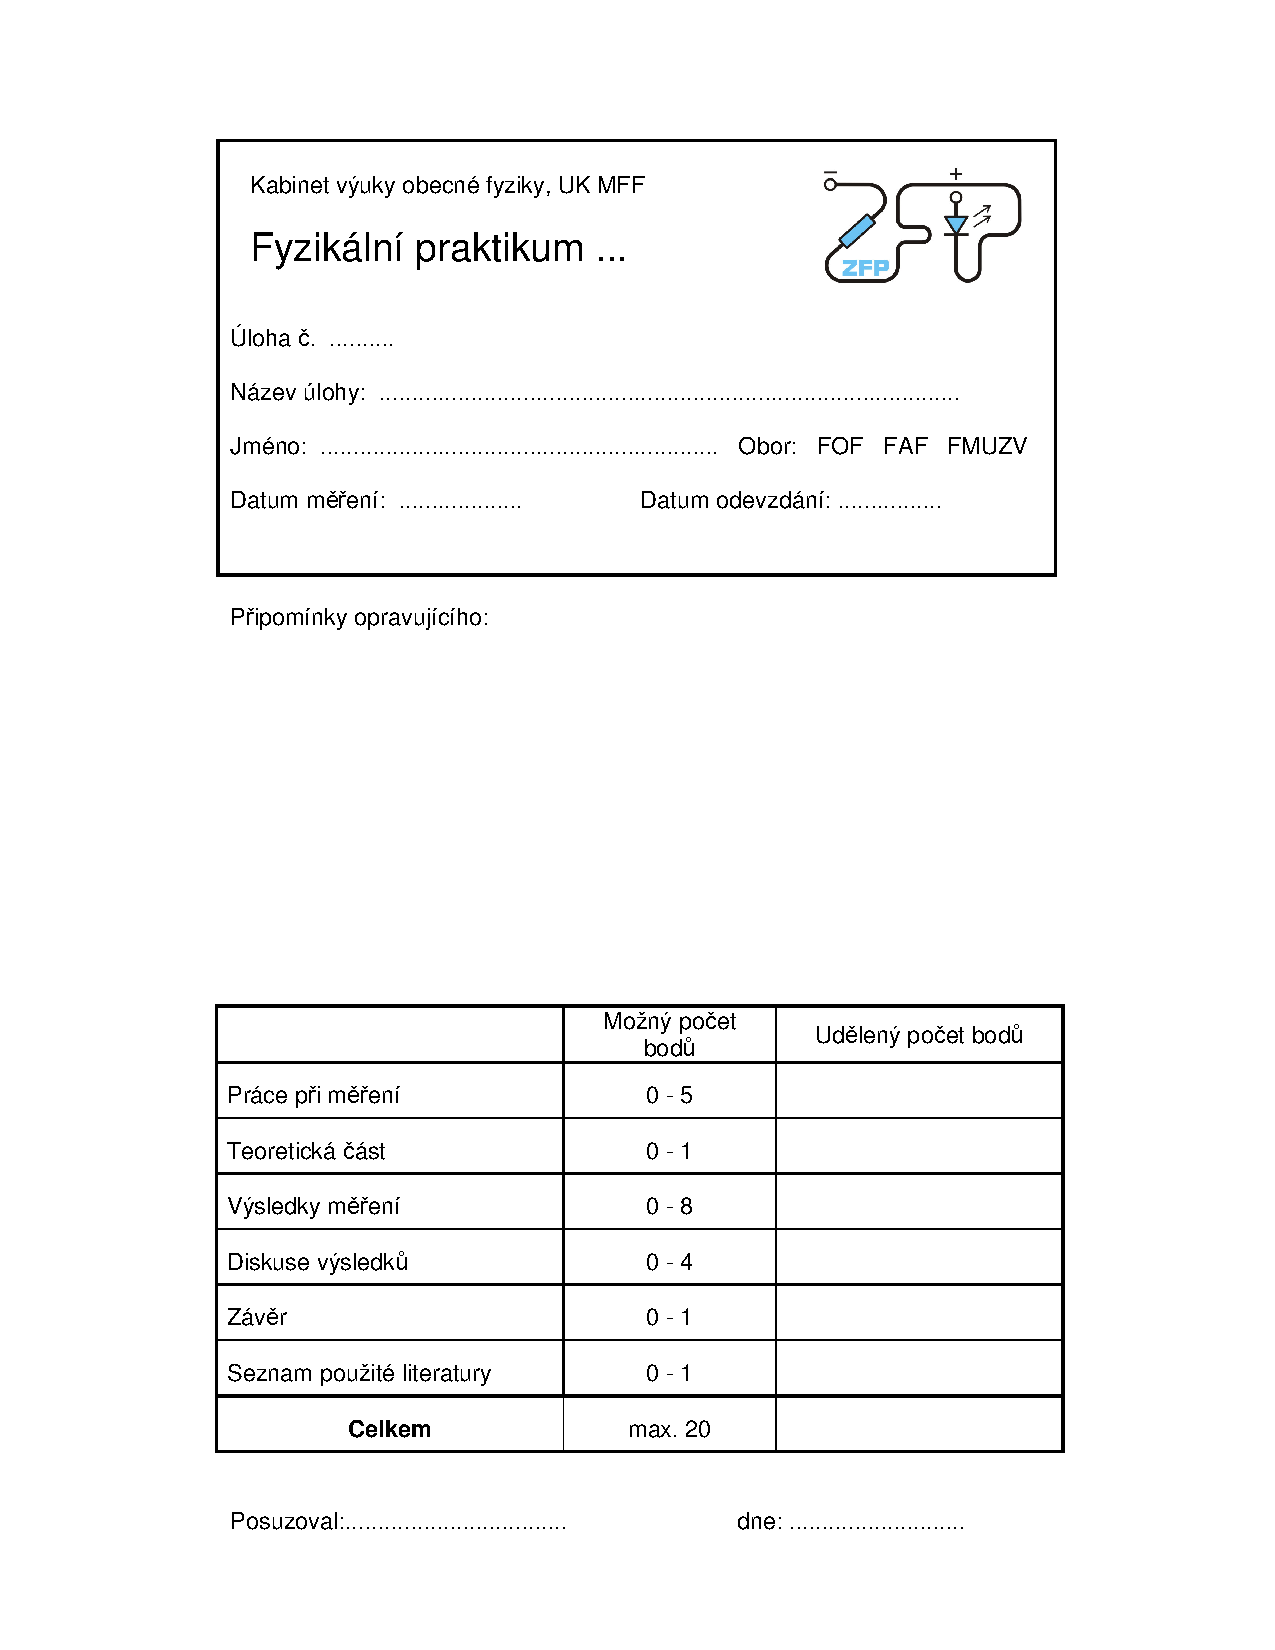
\includepdf[pages={1}]{./graficos/titlelist.pdf}
\end{titlepage}

\section*{Pracovní úkoly}
\begin{enumerate}
\item Pootáčením baňky nastavte elektronový paprsek kolmo k magnetickému poli. Přitom si všímejte, že pokud není elektronový paprsek přesně kolmý k magnetickému poli, tvoří jeho dráha v experimentálním prostoru šroubovici s konstantním stoupáním.
\item Pro celkové urychlovací napětí $U_c$ elektronového svazku v rozmezí od 150 do \SI{350}{\volt} určete magnetizační proudy $I_m$ potřebné k tomu, aby byl průměr kruhové dráhy svazku 40, 60, 80 a \SI{100}{\mm}. Vhodnou volbou dílčích urychlujících napětí $U_1$ a $U_2$ docilujte co nejlepší fokusaci pozorovaného elektronového svazku. Pro každý průměr dráhy naměřte alespoň 10 hodnot.
\item Sestrojte graf závislostí $U_c$ na druhé mocnině $I_m$ pro jednotlivé průměry dráhy svazku. Regresí určete měrný náboj elektronu pro každý průměr dráhy. Diskutujte vliv průměru dráhy svazku na chybu určení $e/m_e$ s přihlédnutím k nejistotě jejího určení.


\end{enumerate}

%Teoretická část
\section*{Teoretická část}
Poměr náboje elektronu $e$ a jeho hmotnosti $m_e$ nazýváme měrný náboj elektronu $e/m_e$.

Pokud elektron letí rychlostí $v$ v homogenním magnetickém poli, jehož směr je kolmý na pohyb elektronu, začne elektron vlivem Lorentzovy síly vykonávat kruhový pohyb o poloměru $r$
\begin{equation} 
m_e  \frac{v^2}{r} = evB \,.
\end{equation}
Pokud je elektron urychlen napětím $U$, má kinetickou energii
\begin{equation}
\frac{1}{2}m_e v^2 = eU \,.
\end{equation}

Dosazením dostáváme měrný náboj \cite{skripta}
\begin{equation} \label{e:mernynaboj}
\frac{e}{m_e} = \frac{2U}{r^2 B^2} \,.
\end{equation}

Pro různá fixovaná $r$ budeme měřit závislost $U(B)$ urychlovacího napětí potřebného k dosažení poloměru dráhy $r$ na velikosti pole $B$.

Magnetické pole budeme realizovat dvojicí cívek v Helmholtzově uspořádání. Pokud do cívek pustíme proud $I_m$, bude magnetická indukce v rovině pohybu elektronů
\begin{equation}
B=\frac{8\mu_0}{5\sqrt{5}} \frac{N I_m}{\rho_0} \,.
\end{equation}
Po dosazení hodnot z \cite{skripta} dostáváme 
$B=(I_m/\SI{5}{\ampere}) \cdot \SI{3.46}{\milli\tesla}$, což se shoduje s hodnotou v \cite{skripta}. Té věříme více, protože předpokládáme, že je změřená.
Dále používáme hodnotu z \cite{skripta}
\begin{equation}
B=(I_m/\SI{5}{\ampere}) \cdot \SI{3.5}{\milli\tesla} = \alpha I_m \qquad \text{, kde }\, \alpha=\frac{\SI{3.5}{\milli\tesla}}{\SI{5}{\ampere}} \,.
\end{equation}
Rozdíl těchto hodnot nám poskytl odhad systematické chyby, standardní odchylku $\alpha$ odhadujeme na \SI{1}{\percent} (po započtení nehomogenity, viz \cite{skripta}). Předpokládáme však, že je závislost skutečně dobře lineární a tato konstanta se pro různé $I_m$ nemění a měříme pořád přibližně na stejném místě, jinými slovy tato chyba se projeví až v konečném výsledku $e/m_e$.

Měřenou závislost $U(B)$ budeme ve skutečnosti měřit jako $U(I_m)$.
\begin{equation} \label{e:zavislost}
U=\frac{1}{2} \frac{e}{m_e} r^2 \alpha^2 I_m^2
\end{equation}

%Výsledky měření
\section*{Výsledky měření}
Měřili jsme závislost $U(I_m)$ pro čtyři různé $r$, viz tabulka \ref{t:vysledky}.
Závislost jsme fitovali afinní funkcí (k \eqref{e:zavislost} jsme přidali $+b$) v proměnné $I_m^2$. Určili jsme pro každý průměr velikost měrného náboje (systematická chyba je \SI{1}{\percent}, viz \emph{Teoretický úvod}, statistická chyba je chyba fitu)
\begin{align*}
        (e/m_e)_{d=\SI{40}{\mm}} &= \chyba{1.59}{0.03}{0.02} \qquad &, b &= \SI{21}{\volt}\\
        (e/m_e)_{d=\SI{60}{\mm}} &= \chyba{1.61}{0.04}{0.02} \qquad &, b &= \SI{51}{\volt}\\
        (e/m_e)_{d=\SI{80}{\mm}} &= \chyba{1.66}{0.03}{0.02} \qquad &, b &= \SI{51}{\volt}\\
        (e/m_e)_{d=\SI{100}{\mm}} &= \chyba{1.70}{0.02}{0.02} \qquad &, b &= \SI{46}{\volt}\\
\end{align*}
Zprůměrováním hodnot dostáváme $(\num[separate-uncertainty=true]{1.64(7)})\cdot\SI{e11}{\coulomb\per\kg}$. Chybu jsme určili součtem přes čtverec statistické chyby dané rozptylem hodnot a průměrné chyby každé z nich.


Chybu měřeného proudu $I_m$ odhadujeme vzhledem ke specifikům přístroje na \SI{0.03}{\ampere}. Chybu měřeného napětí odhadujeme vzhledem ke kolísání hodnot na displeji na \SI{0.5}{\volt}.


\begin{tabulka}[htbp]
\centering
\begin{tabular}{cc|cc|cc|cc}
\multicolumn{2}{c|}{$d=\SI{40}{\mm}$} & \multicolumn{2}{c|}{$d=\SI{60}{\mm}$} &\multicolumn{2}{c|}{$d=\SI{80}{\mm}$} & \multicolumn{2}{c}{$d=\SI{100}{\mm}$} \\
$U$ (\si{\volt}) & $I_m$ (\si{\ampere}) & $U$ (\si{\volt}) & $I_m$ (\si{\ampere}) & $U$ (\si{\volt}) & $I_m$ (\si{\ampere}) & $U$ (\si{\volt}) & $I_m$ (\si{\ampere}) \\ \hline 
174,4 & 3,10 & 183,0 & 1,90 & 184,7 & 1,41 & 170,8 & 1,09 \\ 
190,4 & 3,33 & 201,4 & 2,04 & 197,7 & 1,52 & 190,1 & 1,18 \\ 
211,0 & 3,48 & 221,3 & 2,20 & 212,1 & 1,57 & 210,9 & 1,25 \\ 
229,9 & 3,68 & 240,7 & 2,34 & 230,4 & 1,67 & 230,0 & 1,33 \\ 
251,6 & 3,84 & 261,0 & 2,47 & 249,4 & 1,76 & 252,0 & 1,41 \\ 
272,4 & 4,05 & 274,7 & 2,51 & 270,9 & 1,85 & 270,0 & 1,48 \\ 
290,2 & 4,18 & 288,3 & 2,60 & 291,0 & 1,93 & 292,8 & 1,54 \\ 
311,3 & 4,29 & 311,1 & 2,70 & 311,8 & 2,01 & 307,7 & 1,59 \\ 
329,8 & 4,45 & 330,3 & 2,79 & 329,8 & 2,07 & 329,1 & 1,65 \\ 
354,0 & 4,62 & 354,1 & 2,91 & 354,1 & 2,15 & 354,2 & 1,71 \\ 
\end{tabular}
\caption{Naměřená závislost $U(I_m)$ pro různé $d$}
\label{t:vysledky}
\end{tabulka}

\begin{graph}[htbp] 
\centering
\import{datos/}{UI.tex}
\caption{Naměřená závislost $U(I_m)$ pro různé $r$}
\label{g:vysledky}
\end{graph}


%Diskuze výsledků
\section*{Diskuze}
Fit závislosti $U(I_m)$ je na pohled velmi dobrý (viz graf \ref{g:vysledky}).

Námi změřená hodnota se přibližně shoduje s \SI{1.7e11}{\coulomb\per\kg} uvedenou v \cite{skripta}. Doporučená hodnota Národním institutem standardů a technologie z roku 2014 je přibližně \SI{1.76e11}{\coulomb\per\kg}.

Svazek měl nenulovou šířku a bylo obtížné zajistit, aby měl přesně žádoucí poloměr. Nejvíce se to projevilo při nízkých poloměrech a nízkých proudech. 

%Závěr
\section*{Závěr}


\printbibliography[title={Seznam použité literatury}]

\end{document}